\documentclass{beamer}
\mode<presentation>{\usetheme{DUR}}
\usepackage{amsmath}
\usepackage{cleveref}
\usepackage{wrapfig}
\usepackage[orientation=landscape,size=a2,scale=1.4,grid,debug]{beamerposter}

\newcommand{\defn}[1]{\textit{\color{ETH10}#1}}

\title{Determining Insurance Risk}
\author[Ben Willis]{Ben Willis\\\normalsize{ Supervised by: Dr Matthias Troffaes}}
\institute{Durham University}
\date{\today}
\begin{document}
\begin{frame}
\begin{columns}
	\begin{column}{0.30\paperwidth}

		\begin{block}{Insurance Data Set}

			Classifiers have many applications in the finance industry ranging from financial trading to credit card fraud detection.
			We will study the problem of determining the risk on insuring an auto mobile. \vspace{0.5em}

			\begin{center}
				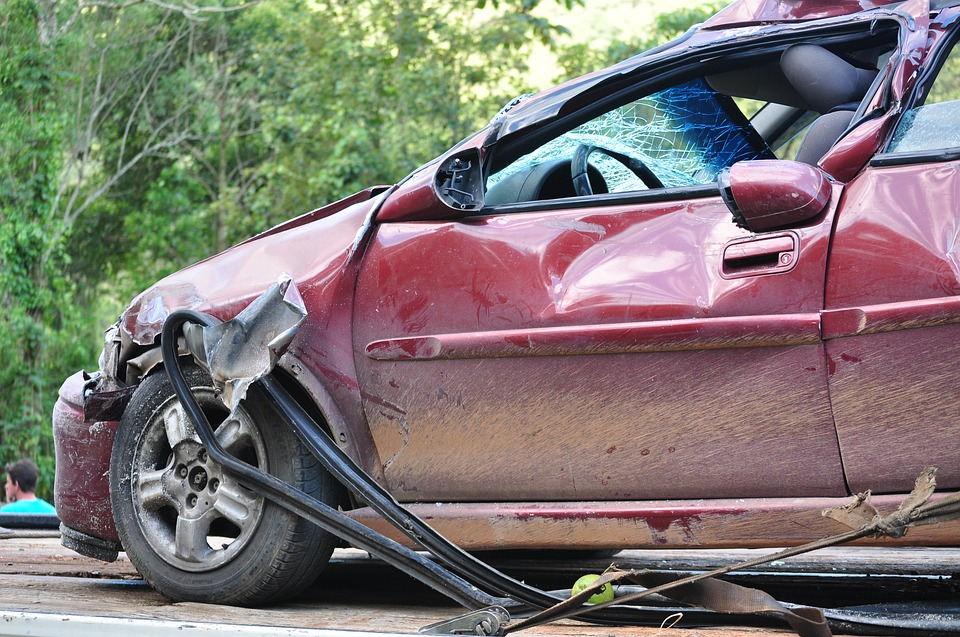
\includegraphics[width=.4\textwidth, keepaspectratio]{img/crash}
			\end{center}

			We will analyse a data set containing the technical attributes of 205 vehicles as well an expert's insurance risk rating.
			This rating is on an integer scale of -2 to 3 with 3 be most risky and -2 being least risky \cite{Automobile}.

			\begin{center}
				\begin{tabular}{l c c c c|c}
					Make       & Length & $\dots$ & Horsepower & Price & Risk \\
					\hline
					Volvo      & 188.8  & $\dots$ & 114        & 12940 & -2   \\
					Audi       & 192.7  & $\dots$ & 110        & 18920 & 2    \\
					Mitsubishi & 172.4  & $\dots$ & 116        & 9279  & 1    \\
					Audi       & 176.6  & $\dots$ & 115        & 17450 & ?
				\end{tabular}
			\end{center}

			We want to be able to accurately predict the risk of a vehicle given its technical information.
		\end{block}

		\begin{block}{Naive Bayes Classifier}
			The \defn{naive Bayes classifier} is a simple probabilistic approach to this classification problem. We are interested in the probability of an auto mobile with attributes $\mathbf{a}$ having risk rating $c$ i.e. $P(c \mid \mathbf{a})$. Using Bayes theorem we can rewrite this as:
			\begin{equation}\label{bayes theorem}
				P(c \mid \mathbf{a}) = \frac{P(c)P(\mathbf{a} \mid c)}{P(\mathbf{a})}
			\end{equation}
			We can use of the \defn{naivety assumption} to simplify the problem.
			The naivety assumptions states that each attribute is conditionally independent given the class.
			We can therefore write the probability of observing an object with attributes $a_1, \dots\ a_k$ given it has risk rating $c$ as:
			\begin{equation} \label{naivety}
				P(\mathbf{a} \mid c) = \prod_{i=1}^k P(a_i \mid c)
			\end{equation}
			Using \cref{bayes theorem,naivety} and noting $P(\mathbf{a})$ does not depend on $c$ we can write:
			\begin{equation}
				P(c \mid \mathbf{a}) \propto P(c)\prod_{i=1}^{k}P(a_i \mid c)
			\end{equation}
			One way to assign a risk rating to a vehicle with attributes $\mathbf{a}$ is to choose the rating which maximises $P(c \mid \mathbf{a})$:
			
			\begin{equation} \label{map_estimate}
				\hat c = \arg\max_{c \in \mathcal{C}} P(c)\prod_{i=1}^{k}P(a_i \mid c)
			\end{equation}
			This is known as the \defn{maximum a posteriori estimate}.
		\end{block}

	\end{column}

	\begin{column}{0.30\paperwidth}

		\begin{block}{Likelihood Function}
			Now that we have our decision mechanism we need to estimate the required probabilities. We parametrise these probabilities:
			\begin{description}
				\item[\theta_c] Chance of a vehicle having risk $c$
				\item[\theta_{a_i \mid c}] Chance of a vehicle having attribute $a_i$ given that it has risk $c$
			\end{description}\vspace{0.5em}

			Given $N$ observations we denote the observed frequencies:
			\begin{description}
				\item[n(c)] Number of vehicles with risk $c$
				\item[n(a_i, c)] Number of vehicles with attribute $a_i$ and risk $c$
			\end{description}
			Note that $\sum_{c \in \mathcal{C}}n(c) = N$ and $\sum_{a_i \in \mathcal{A}_i}n(a_i, c) = n(c)$.\vspace{0.5em}

			The likelihood function for these theta chances given our observations is given by \cite{Zaffalon01}:
			\begin{equation} \label{likelihood}
				l(\mathbf{\theta} \mid \mathbf{n}) \propto \prod_{c \in \mathcal{C}} \left[ \theta_c^{n(c)} \prod_{i=1}^k \prod_{a_i \in \mathcal{A}_i} \theta_{a_i \mid c}^{n(a_i, c)} \right]
			\end{equation}
		\end{block}

		\begin{block}{Prior Distribution}
			We choose the following to be the prior distribution to our likelihood:
			\begin{equation} \label{prior}
				f(\mathbf{\theta} \mid \mathbf{t}, s) \propto \prod_{c \in \mathcal{C}} \left[ \theta_c^{st(c) - 1} \prod_{i=1}^k \prod_{a_i \in \mathcal{A}_i} \theta_{a_i \mid c}^{st(c, a_i) - 1} \right]
			\end{equation}
			where $s>0$ and $t(\cdot)$ are such that:
			\begin{equation}
				\sum_{c \in \mathcal{C}} t(c) = 1 \qquad \sum_{a_i \in \mathcal{A}_i} t(a_i, c) = t(c)  \ \forall \  i, c \qquad t(a_i, c) & > 0  \ \forall  \ i, a_i, c
			\end{equation}
			This distribution is the conjugate prior for our likelihood so the posterior distribution is in the same form as the likelihood. If the prior has hyper parameters $st(\cdot)$ the posterior will have hyper parameters $st(\cdot) + n(\cdot)$.\vspace{0.5em}

			Note that $t(c)$ and $t(a_i , c)$ represent our prior beliefs about $P(c)$ and $P(a_i \mid c)$. We want our prior to be as uninformative as possible so we set it to be uniform \cite{laplace1812} by choosing parameters:
			\begin{equation}
				s = 1 \qquad t(c) = \frac{1}{|\mathcal{C}|} \qquad t(a_i, c) = \frac{1}{|\mathcal{A}_i||\mathcal{C}|}
			\end{equation} 
		\end{block}

		\begin{block}{\small References}
			{\footnotesize
			\bibliography{refs}{}}
			\bibliographystyle{abbrv}
		\end{block}
		
	\end{column}

	\begin{column}{0.30\paperwidth}

		\begin{block}{Estimating Probabilities}
			To use the naive Bayes classifier we need to estimate the probabilities involved.\vspace{0.5em}

			One way is by choosing the theta values which maximise the likelihood. These are the \defn{maximum likelihood estimates} and are given by:
			\begin{equation}\label{mles}
				\hat{\theta}_c = \frac{n(c)}{N} \qquad
				\hat{\theta}_{a_i \mid c} = \frac{n(a_i, c)}{n(c)}
			\end{equation}\vspace{0.5em}

			Alternatively we can multiply our likelihood by our prior and take the expectation of the posterior. These estimates are \cite{Zaffalon01}:
			\begin{align}
				E(\theta_c \mid \mathbf{n},s,\mathbf{t}) & = \frac{n(c) + st(c)}{N + s} = \hat{\theta}_c \\
				E(\theta_{a_i \mid c} \mid \mathbf{n},s,\mathbf{t}) & = \frac{n(c) + st(a_i, c)}{N + st(c)} = \hat{\theta}_{a_i \mid c}
			\end{align}
		\end{block}

		\begin{block}{Application}
			To apply our classifier to the insurance data set we must first discretize continuous variables. Also we have no mechanism for dealing with missing values so we must discard any vehicles which are missing technical information.\vspace{0.5em}

			We will measure three metrics:
			\begin{description}
				\item[Accuracy] The percentage or correct risk assignments.
				\item[Random Assignments] The percentage or objects for which $P(c \mid \mathbf{a}) = 0$ for all $c$, in these cases the classifier randomly assigns a class.
				\item[Mean Squared Error (MSE)] The average squared difference between the assigned class and true class; this metric indicates closeness.
			\end{description}\vspace{0.5em}
		\end{block}

		\begin{block}{Results}
			The measurements for the three metrics for each estimate are given below.
			\begin{center}
				\begin{tabular}{ l|c c c c c c }
					                      & Accuracy & MSE   & Random Assignments\\
					\hline
					Maximum Likelihood    & 59.95\%  & 2.823 & 22.45\% \\
					Posterior Expectation & 68.17\%  & 0.689 & 0\%
				\end{tabular}
			\end{center}
			Overall using the posterior expectation is more accurate than than using the maximum likelihood estimates. It also assigns risks which are closer to the true value and it never randomly assigns classes.\vspace{0.5em}

			The next step is to consider how sensitive our classifier is to changes in our prior distribution. We could also look at other decision mechanisms for assigning risk and ways to deal with missing values.
		\end{block}

	\end{column}
\end{columns}
\end{frame}
\end{document}